\documentclass[11pt]{article}
\ifdefined\pdfinfoomitdate\pdfinfoomitdate=1\fi
\ifdefined\pdftrailerid\pdftrailerid{}\fi
\ifdefined\pdfsuppressptexinfo\pdfsuppressptexinfo=15\fi
\ifdefined\pdfgentounicode
  \pdfgentounicode=1
  \input{glyphtounicode}
  \input{glyphtounicode-cmex}
\fi
\usepackage[T1]{fontenc}
\usepackage[utf8]{inputenc}
\usepackage{lmodern,microtype,amsmath,amssymb,amsthm,mathtools}
\usepackage[margin=1in]{geometry}
\usepackage{enumitem,tikz,needspace}
\usetikzlibrary{arrows.meta,positioning}
\usepackage{xurl}
\usepackage[colorlinks=true,linkcolor=blue,citecolor=blue,urlcolor=blue]{hyperref}
\hypersetup{pdftitle={Tree Constructions for the l1 Distortion of Binary Edit Distance},pdfauthor={OpenAI},bookmarksdepth=2}
\newtheorem{theorem}{Theorem}[section]
\newtheorem{proposition}[theorem]{Proposition}
\newtheorem{lemma}[theorem]{Lemma}
\newtheorem{corollary}[theorem]{Corollary}
\theoremstyle{definition}\newtheorem{definition}[theorem]{Definition}
\theoremstyle{remark}\newtheorem{remark}[theorem]{Remark}
\newcommand{\ED}{\operatorname{ED}}
\newcommand{\LCS}{\operatorname{LCS}}
\newcommand{\dist}{\operatorname{dist}}
\newcommand{\E}{\mathbb E}
\newcommand{\Prb}{\mathbb P}
\newcommand{\T}{\mathbb T}
\newcommand{\Z}{\mathbb Z}
\newcommand{\R}{\mathbb R}
\newcommand{\ellone}{\ell_1}
\newcommand{\one}{\mathbf 1}
\newcommand{\enc}{\operatorname{enc}}
\newcommand{\wt}{\operatorname{wt}}
\DeclareMathOperator{\ord}{ord}
\title{Tree Constructions for the $\ell_1$ Distortion\\
of Binary Edit Distance}
\author{OpenAI}
\date{September 27, 2026}
\begin{document}
\maketitle
\begin{abstract}
We give two independent constructions of binary words of one length at
most $d$ whose ordinary edit-distance metrics require $\ell_1$ distortion
$\exp(\Omega(\sqrt{\log d\,\log\log d}))$ for every sufficiently large $d$.
We also prove a constant-distortion binary conversion for one prescribed
input length. Together with the companion upper embedding theorem, these
lower bounds determine the order of logarithmic distortion uniformly over
finite alphabets with at least two symbols.
\end{abstract}
\setcounter{tocdepth}{1}
\tableofcontents
\section{Introduction}\label{sec:introduction}

An insertion or deletion changes the positions of every later symbol in
a word. A long interval can therefore move at small edit cost even when
many positions change. This tension between order and inexpensive shifts
is central to the question studied here: how faithfully can one represent
the edit distances of an entire set of words by distances in $\ellone$?

We use ordinary edit distance $\ED(x,y)$: the minimum number of
single-symbol insertions, deletions and substitutions taking $x$ to $y$,
each with cost one. For a finite alphabet $\Sigma$ with at least two
symbols and an integer
$d\geq1$, let $\Sigma^{\leq d}$ be the set of words of length at most
$d$, including the empty word. The cap constrains the words in the
domain; an edit script computing their distance may pass through words
of any finite length.

For a finite metric space $(X,\rho)$ with at least two points and an
injective map $f:X\to\ellone$, where $\ellone$ is the space of absolutely
summable real sequences, define
\[
 \dist(f)=
 \left(\max_{x\ne y}\frac{\|f(x)-f(y)\|_1}{\rho(x,y)}\right)
 \left(\max_{x\ne y}\frac{\rho(x,y)}{\|f(x)-f(y)\|_1}\right).
\]
Let $c_1(X,\rho)$ be the infimum of $\dist(f)$ over such maps, and put
$E_\Sigma(d)=c_1(\Sigma^{\leq d},\ED)$. No restriction is imposed on
the dimension of the image or on the computation of the map. Throughout
the paper, logarithms in asymptotic estimates are natural unless a base
is written explicitly.

We prove the following lower bound in two independent ways. Each proof
uses a tree to combine inexpensive shifts with a displacement that no
alignment can hide.

\begin{theorem}[Binary lower bound]\label{thm:binary}
There are an absolute constant $c>0$ and an integer $d_0$ such that,
for every integer $d\geq d_0$, there exist an integer $1\leq n\leq d$ and a
finite set $\mathcal W\subseteq\{0,1\}^n$ with $|\mathcal W|\geq2$
satisfying
\[
 c_1(\mathcal W,\ED)
 \geq \exp\!\left(c\sqrt{\log d\,\log\log d}\right).
\]
\end{theorem}

The words in a witness all have the same length, although that length
may depend on the cap $d$. At tree depth $k$, each construction
produces logarithmic distortion of order at least $k\log k$ and
logarithmic word length of order $k^2\log k$. Balancing these two scales
gives Theorem~\ref{thm:binary} for every sufficiently large cap, not just
for a subsequence of caps.

The lower bound is proved here without a companion input. The uniform
upper embedding theorem of the finite-circle companion, stated precisely
in Section~\ref{sec:consequences}, then gives
\[
 \log E_\Sigma(d)=\Theta\!\left(\sqrt{\log d\,\log\log d}\right)
\]
with constants independent of the finite alphabet $\Sigma$. This is a
matching exponential scale, not a constant-factor estimate for
$E_\Sigma(d)$ itself.

\subsection{History and the embedding question}

The single-symbol error model is classical in coding and sequence
comparison. Levenshtein studied binary codes correcting insertions and
deletions \cite{Levenshtein1966}, and Wagner and Fischer formulated
string correction through increasing partial alignments
\cite[Sections~3 and~5]{WagnerFischer1974}. An embedding asks for one set of
coordinates that represents every pair in a domain. It is a different
task from estimating the distance of one given pair of words.
For supplied pairs of binary words, \cite[Theorem~1.1]{OpenAIEditApprox2026}
gives a randomized approximation scheme with almost-linear worst-case
expected time for each fixed rational accuracy.

Ostrovsky and Rabani proved an $\ellone$ distortion bound
$\exp(O(\sqrt{\log n\,\log\log n}))$ for binary words of a fixed length
$n$ \cite{OstrovskyRabani2007}. Their recursion compares overlapping
substrings and represents their distributions in smaller metric spaces.
They also noted extensions to larger alphabets and varying lengths.
For the upper bound used at the end of this paper, the companion uniform
upper embedding theorem
\cite[Uniform upper embedding theorem]{OpenAIUniformUpper2026}
gives the full quantitative statement on
$\Sigma^{\leq d}$ with constants independent of the finite alphabet.

On the lower-bound side, Andoni, Deza, Gupta, Indyk and Raskhodnikova
realized complete bipartite graph metrics in binary edit distance and
obtained $\ellone$ distortion approaching $3/2$
\cite[Section~2 and Theorem~3.1]{AndoniDezaGuptaIndykRaskhodnikova2003}.
Their witness uses three adjacent word lengths.
Khot and Naor developed Fourier methods for
nonembeddability and obtained an edit-distance lower bound of
$(\log n)^{1/2-o(1)}$ for binary words of a fixed length
\cite{KhotNaor2006}. Their insertion--deletion
metric and the ordinary metric used here differ by at most a factor of
two. Krauthgamer and Rabani then proved an $\Omega(\log n)$ lower bound
for binary words of length $n$ \cite[Theorem~1.3]{KrauthgamerRabani2009}.
Khot and Naor used Boolean noise sensitivity, while Krauthgamer and
Rabani sharpened the obstruction through an influence inequality for
bit flips and cyclic shifts. These cut and shift arguments are
methodological predecessors of the proofs here. A cut records which
pairs a binary coordinate separates, and Fourier coefficients describe
how that separation changes under translations. We prove the particular
translation estimates needed for our trees.

Alphabet reduction also has a substantial history. Schulman and
Zuckerman use separation between long intervals of distinct codewords
in concatenated insertion--deletion codes \cite{SchulmanZuckerman1999},
and synchronization strings protect positions against insertion and
deletion errors \cite{HaeuplerShahrasbi2017}. More directly,
Bhattacharya, Dey, Goldenberg and Kouck\'y state a map on all finite
words with an insertion--deletion guarantee normalized by the sum of
the word lengths, for pairs of positive total length. The block
substitution used to prove their stated theorem has logarithmic width
and, for a fixed error parameter, a constant target alphabet
\cite[Theorem~3; full version, Section~3.2.1 and Lemma~3.3]{BhattacharyaDeyGoldenbergKoucky2024}.
For equal-length inputs, their stated normalized guarantee, combined
with the elementary delimiter construction below, gives a binary
reduction with logarithmic width and absolute distortion. Our lower
proofs do not use that result. They use the short delimiter code, whose
width-dependent loss is harmless at the tree scale; the appendix gives
a separate constant-distortion code for one prescribed word length.
For comparison, the isometric Hamming-to-edit embedding of Bhattacharya
et al.\ \cite[Theorem~7]{BhattacharyaEtAl2026} starts from a different
input metric. The conversions proved here compare edit distance on the
source words with edit distance on their binary encodings.

\subsection{Two independent tree proofs}

Both constructions use an ordered tree. A leaf has a state coordinate
and produces a symbol carrying its leaf label. An internal node produces
a long list of rows, each containing its child words in their fixed
order. Advancing the row index deletes a few rows at one end and inserts
a few at the other, so it is inexpensive. A distinguished second shift
must instead separate the words even when an alignment crosses row
boundaries.

The shared alignment lemma in Section~\ref{sec:preliminaries} handles
this difficulty. Leaf labels preserve child indices, not row indices.
An unsplit source row loses symbols because its child words are
separated from the corresponding target words. A split source row
forces a long unmatched target interval between consecutive matches.
The intervals charged by different source rows are disjoint. Thus
separation in every comparison of two rows implies separation of the
whole words, without assuming that row boundaries match.

The two constructions arrange the shifts differently.
In the finite tree of Section~\ref{sec:finite}, a child's period is its
parent's period times a new prime. At an internal node, a vector $u_v$
advances rows and a multiple $w_v$ has the parent period. The distinct
prime factors prevent a difference of row indices from cancelling the
distinguished shift in too many children. This gives a deterministic
separation proof on a finite group. For a Fourier character, activity at
a node with few active children has a short period and is detected by
an average of inexpensive row shifts. A character escaping every such
test must be active on many leaves; individual leaf changes then bound
its contribution. The section closes with binary witnesses for every
large cap.

The circle tree in Sections~\ref{sec:torus-construction}
and~\ref{sec:torus-fourier} uses quantized phases instead of finite
residues. Random prime lists and coefficients make the root half-turn
separate every base phase. The probabilistic assertion is only for one
fixed shift; the all-phase conclusion follows deterministically from
the alignment lemma. In its Fourier argument, tiny rotations detect
large integer frequency sums and rational row shifts detect failed
prime congruences. When both tests fail, divisibility forces every
nonzero sum to continue through many children. This supplies the second
binary proof without using the finite tree.

Both routes use the same elementary delimiter code from
Section~\ref{sec:preliminaries}. Its distortion loss grows with the
block width, but that width is only $O(k\log k)$ here and does not
change the logarithmic lower-bound scale. Appendix~\ref{sec:code}
proves a stronger, separate alphabet-conversion theorem: for words of
one prescribed length $M$ over at most $M$ letters, blocks of width
$M^2$ preserve edit distance up to scale and an absolute factor $804$.
Its proof is independent of both trees, and neither headline lower
bound requires this stronger conversion.

\section{Edit deficits, ordered rows and binary transfer}
\label{sec:preliminaries}

Both trees need four elementary tools. Subsequence deficits and an
alignment lemma turn separation of child blocks into separation of
whole words, even when matches cross row boundaries. A cut
representation permits the later Fourier estimates, and a prime count
supplies the periods. Finally, a short binary code transfers either
tree's obstruction to binary words with a controlled width loss.

\subsection{Subsequence matchings}

A common subsequence matching of words $x=x_1\cdots x_a$ and
$y=y_1\cdots y_b$ is a list of pairs
$(i_1,j_1),\ldots,(i_s,j_s)$ whose two index lists are strictly
increasing and for which $x_{i_t}=y_{j_t}$ for every $t$. Its largest
possible size is $\LCS(x,y)$. The insertion--deletion distance is
\[
 \Delta(x,y)=|x|+|y|-2\LCS(x,y).
\]
Indeed, symbols of $x$ that survive an insertion--deletion script form
a common subsequence; conversely, retaining a longest common subsequence
and deleting and inserting the remaining symbols attains this value.
Replacing each substitution by one deletion and one insertion gives
\begin{equation}\label{eq:metric-conversion}
 \ED(x,y)\leq\Delta(x,y)\leq2\ED(x,y).
\end{equation}
For words of equal length $n$, put $r_n(x,y)=n-\LCS(x,y)$. Thus
\begin{equation}\label{eq:deficit}
 r_n(x,y)\leq\ED(x,y)\leq2r_n(x,y).
\end{equation}
A matching of size $n-E$ between two length-$n$ words leaves exactly
$E$ unmatched positions on each side.

\subsection{The common alignment lemma}

Suppose each row consists of one block from each of several pairwise
disjoint alphabets, in the same order. An equal-symbol match must then
join blocks with the same index, although their row indices can differ.
Products of words in the next lemma mean concatenation in increasing
index order.

\Needspace{15\baselineskip}
\begin{lemma}[Rows with ordered tags]\label{lem:tagged}
Let $T,B\geq1$ and $m\geq2$ be integers, and let
$\Gamma_1,\ldots,\Gamma_m$ be pairwise disjoint alphabets. For
$1\leq a,b\leq T$ and $1\leq i\leq m$, take
$X_{a,i},Y_{b,i}\in\Gamma_i^B$, and define
\[
 X=\prod_{a=1}^T(X_{a,1}\cdots X_{a,m}),\qquad
 Y=\prod_{b=1}^T(Y_{b,1}\cdots Y_{b,m}),\qquad N=TmB.
\]
Suppose $d\geq0$ is real and
\begin{equation}\label{eq:local-tagged}
 \sum_{i=1}^m r_B(X_{a,i},Y_{b,i})\geq d
 \qquad(1\leq a,b\leq T).
\end{equation}
With $g=(m-1)B$, one has
\begin{equation}\label{eq:tagged-result}
 r_N(X,Y)\geq\frac{Tdg}{d+g}
 \geq\frac T2\min(d,g).
\end{equation}
In particular, $d\leq g$ implies $r_N(X,Y)\geq Td/2$.
\end{lemma}

\begin{proof}
Fix an increasing matching and let $E$ be its unmatched count on either
side. Call a source row split if it has matches in at least two target
rows, and let $s$ be the number of split source rows.

A source row that is not split and has matches sends them all into one
target row, say $b$. The disjoint alphabets confine matches from its
block $i$ to block $i$ in that target row. The restriction of the
matching to those two blocks has size at most their $\LCS$, even if
other source rows also use the target block. Condition
\eqref{eq:local-tagged} therefore leaves at least $d$ unmatched source
positions in this row. A source row with no matches loses all $mB$
positions, again at least $d$, since \eqref{eq:local-tagged} implies
$d\leq mB$. The nonsplit rows are disjoint, so
\begin{equation}\label{eq:tagged-unsplit}
 E\geq d(T-s).
\end{equation}

For a split source row, list its matches in order and choose two
consecutive entries at a transition between target rows. They are also
consecutive in the entire matching: every source position between them
lies in the same source row, so an intervening global match would have
appeared in its list. Let $i,i'$ be their source block indices. Their
order gives $i\leq i'$, and disjoint alphabets give the same two block
indices in the target. Between their target positions lie at least
\[
 (m-i+i'-1)B\geq(m-1)B=g
\]
positions in complete blocks. This is the count for adjacent target
rows; intervening rows only increase it. All positions in that open
target interval are unmatched, because the selected matches are
globally consecutive. The intervals selected for different source rows
are disjoint by strict monotonicity of the matching. Hence
\begin{equation}\label{eq:tagged-split}
 E\geq sg.
\end{equation}

Since $g>0$, \eqref{eq:tagged-split} gives $s\leq E/g$. Substitute this
in \eqref{eq:tagged-unsplit} to obtain
$E\geq d(T-E/g)$, and rearrange:
$E\geq Tdg/(d+g)$. If $d\leq g$, then $dg/(d+g)\geq d/2$; if
$g\leq d$, it is at least $g/2$. These bounds hold for every matching,
including when $d=0$ or $T=1$, and therefore for a longest one.
\end{proof}

The two inequalities in the proof bound the same number $E$ using
different words: nonsplit rows give source losses, and split rows give
target losses. Equal total lengths make the unmatched counts equal.
The fixed order, equal block lengths and disjoint tags supply the
target gaps; no alignment of row boundaries is assumed.
Figure~\ref{fig:tagged-gap} illustrates the gap created by a split row.

\begin{figure}[ht]
\centering
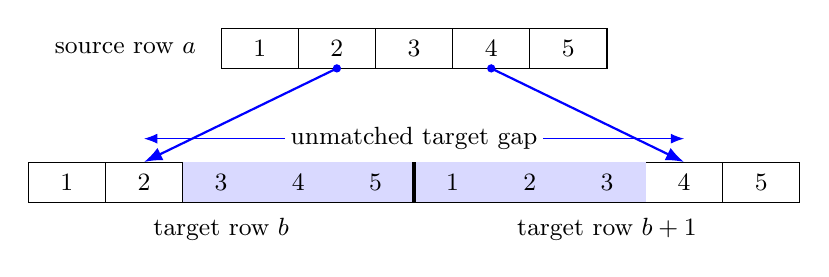
\begin{tikzpicture}[x=0.98cm,y=0.85cm,>=Latex,
 every node/.style={font=\small}]
 \foreach \block in {1,...,5} {
  \draw ({\block+1.5},2) rectangle ({\block+2.5},2.6);
  \node at ({\block+2},2.3) {$\block$};
 }
 \node[anchor=east] at (2.3,2.3) {source row $a$};
 \foreach \block in {1,...,5} {
  \draw ({\block-1},0) rectangle (\block,0.6);
  \draw ({\block+4},0) rectangle ({\block+5},0.6);
 }
 \foreach \block in {3,4,5} {
  \fill[blue!15] ({\block-1},0) rectangle (\block,0.6);
 }
 \foreach \block in {1,2,3} {
  \fill[blue!15] ({\block+4},0) rectangle ({\block+5},0.6);
 }
 \foreach \block in {1,...,5} {
  \node at ({\block-0.5},0.3) {$\block$};
  \node at ({\block+4.5},0.3) {$\block$};
 }
 \draw[very thick] (5,0) -- (5,0.6);
 \node at (2.5,-0.4) {target row $b$};
 \node at (7.5,-0.4) {target row $b+1$};
 \draw[blue,thick,->] (4,2) -- (1.5,0.6);
 \draw[blue,thick,->] (6,2) -- (8.5,0.6);
 \fill[blue] (4,2) circle (1.5pt);
 \fill[blue] (6,2) circle (1.5pt);
 \draw[blue,<->] (1.5,0.95) -- (8.5,0.95);
 \node[fill=white,inner sep=2pt] at (5,0.95) {unmatched target gap};
\end{tikzpicture}
\caption{A split source row in Lemma~\ref{lem:tagged}, with $m=5$.
The two arrows are consecutive matches from source blocks $i=2$ and
$i'=4$. Their target positions lie in different rows, so all positions
between them are unmatched. The six shaded complete blocks contribute
$(m-i+i'-1)B=6B\geq(m-1)B$ positions. The diagram is schematic; target
rows further apart would only enlarge the gap.}
\label{fig:tagged-gap}
\end{figure}


\subsection{Cuts and prime counts}

We record two background facts for both constructions. The first turns
an $\ellone$ distance on a finite set into a nonnegative sum of binary
separation tests. This standard cut description is stated, for example,
in Section~4 of Linial, London and Rabinovich
\cite{LinialLondonRabinovich1995}; the proof below includes a summability
bound for maps with infinitely many coordinates.

\begin{lemma}[Finite cut representation]\label{lem:cuts}
Let $S$ be finite and $f:S\to\ellone$. There are nonnegative finite
weights $a_C$, indexed by nonempty proper subsets $C\subset S$, such that
\[
 \|f(x)-f(y)\|_1
 =\sum_{\varnothing\ne C\subsetneq S}
 a_C|\one_C(x)-\one_C(y)|.
\]
Moreover,
\[
 \sum_{\varnothing\ne C\subsetneq S}a_C
 \leq\sum_{\{x,y\}\subset S,\ x\ne y}\|f(x)-f(y)\|_1,
\]
where the sum on the right is over unordered pairs.
\end{lemma}
\begin{proof}
For each real coordinate $f_j$,
\[
 |f_j(x)-f_j(y)|
 =\int_{\R}|\one_{\{f_j>t\}}(x)-\one_{\{f_j>t\}}(y)|\,dt.
\]
Discard empty and full level sets, which contribute zero, then sum over
coordinates and group the remaining level sets by their subset of $S$.
All terms are nonnegative, so monotone convergence permits this
grouping. Every nontrivial cut separates at least one unordered pair.
Summing the identity over those pairs bounds the total weight of the
nontrivial cuts by the stated finite sum.
\end{proof}

The second fact supplies all primes used below. We use the elementary
binomial-coefficient argument, following the classical prime-product
method found, for example, in Erd\H{o}s \cite{Erdos1932}. Write $\pi(x)$
for the number of primes at most $x$.

\begin{lemma}[Prime supply]\label{lem:primes}
There is an absolute $c>0$ such that
$\pi(x)\geq cx/\log x$ for all sufficiently large real $x$.
Consequently, for all sufficiently large integers $k$, the interval
$[k^4,k^5]$ contains at least $20k^2$ primes and $[k^2,k^3]$ contains
more than $1600k$ primes.
\end{lemma}
\begin{proof}
For an integer $a\geq1$, the largest coefficient in the expansion of
$(1+1)^{2a}$ is the central one, so
$\binom{2a}{a}\geq4^a/(2a+1)$. The exponent of a prime $p$ in this
coefficient is
\[
 \sum_{s\geq1}
 \left(\left\lfloor\frac{2a}{p^s}\right\rfloor
 -2\left\lfloor\frac a{p^s}\right\rfloor\right).
\]
Each summand is zero or one and vanishes for $p^s>2a$. Hence the whole
$p$-power dividing $\binom{2a}{a}$ is at most $2a$, and
$\binom{2a}{a}\leq(2a)^{\pi(2a)}$. Taking logarithms gives
$\pi(2a)\geq c(2a)/\log(2a)$ for large $a$. Taking
$a=\lfloor x/2\rfloor$ yields the asserted lower bound for real $x$.
Finally subtract $\pi(k^4)\leq k^4$ from the lower bound at $k^5$,
and $\pi(k^2)\leq k^2$ from the lower bound at $k^3$. The respective
differences eventually exceed $20k^2$ and $1600k$.
\end{proof}

\subsection{A short binary code}

The trees initially use leaf labels and hence a growing alphabet. The
following code will suffice for both binary lower bounds. It preserves
subsequence deficits from below, while its expansion is at most its
block width. For the tree alphabets that width will be $O(k\log k)$,
small compared with their eventual distortion lower bounds.

\begin{lemma}[Delimiter transfer]\label{lem:delimiter}
Let $\Gamma$ be a finite alphabet of size $A\geq2$, let
$t\geq\lceil\log_2A\rceil$ be an integer, and put $B=2t+3$.
Give the symbols of $\Gamma$ distinct
labels $(a_1,\ldots,a_t)\in\{0,1\}^t$. Let $c(a)$ be the prefix
$110$ followed, in order, by the two-bit words $a_j0$ for
$j=1,\ldots,t$.
Let $\mathcal B$ extend $c$ by concatenation. For every integer
$n\geq0$ and every $x,y\in\Gamma^n$,
\begin{equation}\label{eq:delimiter}
 \frac12r_n(x,y)
 \leq\ED(\mathcal B(x),\mathcal B(y))
 \leq B\ED(x,y).
\end{equation}
\end{lemma}
\begin{proof}
The pattern $11$ occurs in a concatenation only at block starts.
The final zero of each block prevents an additional occurrence across
a boundary. Fix a longest
common subsequence matching of the encoded words, and let $l$ be its
unmatched count on each side.

At most $l$ source blocks contain an unmatched source bit. Among
the fully matched source blocks, consider one whose image is not a
consecutive target interval. Two consecutive bits of that source
block then have matched target positions with a nonempty gap. No target
position in that gap is matched: there is no source position between
the two consecutive source bits. The gaps chosen for different source
blocks are disjoint by monotonicity. Thus at most $l$ additional
source blocks have a nonconsecutive target image.

Every remaining source block is matched to a consecutive target
interval of length $B$. Its initial $11$ starts at a target block
boundary, so the entire block equals that target block. These target
blocks are distinct and occur in increasing order. Their original
letters form a common subsequence of $x,y$ with at least $n-2l$
letters. Hence $r_n(x,y)\leq2l$. By \eqref{eq:deficit}, encoded edit
distance is at least its one-sided deficit $l$, proving the lower
bound. Simulating each original symbol edit by at most $B$ bit edits
gives the upper bound, with no restriction on intermediate lengths.
When $n=0$, both sides are zero.
\end{proof}

By \eqref{eq:deficit}, the lower bound in \eqref{eq:delimiter} is at
least $\ED(x,y)/4$. Consequently, if a finite set of equal-length
words has $\ellone$ distortion at least $D_0$, its encoded image has
distortion at least $D_0/(4B)$: composing an embedding of the encoded
image with $\mathcal B$ incurs at most the factor $4B$.

\section{A finite tree with nested periods}\label{sec:finite}

We first construct words over a finite alphabet that grows with the
tree. At every internal node, one vector advances the rows cheaply and
a multiple of it has a prescribed smaller period. The latter vector
separates words for every state. We then use Fourier analysis to show
that an $\ellone$ map cannot preserve both kinds of displacement with
small distortion. The short binary code from
Lemma~\ref{lem:delimiter} will then complete the first proof of
Theorem~\ref{thm:binary}.

\subsection{Periods and word construction}

Fix a sufficiently large integer $k$ and put
\begin{equation}\label{eq:finite-parameters}
 m=20k,\qquad T=k^{20k}.
\end{equation}
Use the full ordered $m$-ary tree of depth $k$, with root $o$ at depth
zero and children $v1,\ldots,vm$ at each internal node $v$.
By Lemma~\ref{lem:primes}, choose primes
$p_{j,i}\in[k^4,k^5]$ distinct over all pairs
$0\leq j<k$, $1\leq i\leq m$. Nodes at the same depth use the same
list. Define their periods by
\[
 Q_o=2,\qquad Q_{vi}=Q_vp_{j,i}
 \quad\text{when $v$ has depth $j$}.
\]
All these primes are odd for large $k$.

On the finite abelian group
\[
 A=\prod_{u\text{ leaf}}\Z/Q_u\Z
\]
define vectors supported on their respective subtrees:
\begin{equation}\label{eq:finite-vectors}
 \begin{aligned}
 w_u&=e_u &&(u\text{ leaf}),\\
 u_v&=\sum_{i=1}^m w_{vi},\qquad
 R_v=\prod_{i=1}^m p_{j,i},\qquad
 w_v=R_vu_v
 &&(v\text{ internal at depth }j).
 \end{aligned}
\end{equation}
Here $e_u$ increments the coordinate of leaf $u$.

\begin{lemma}[Orders of the node vectors]\label{lem:orders}
For every node $v$, $\ord(w_v)=Q_v$. At every internal node,
\[
 \ord(u_v)=Q_vR_v,\qquad \gcd(Q_v,R_v)=1.
\]
\end{lemma}
\begin{proof}
At a leaf, $e_u$ has order $Q_u$. Suppose the assertion holds at the
children of an internal node $v$. Their vectors have disjoint supports
and orders $Q_vp_{j,i}$, so their sum has order
\[
 \ord(u_v)=\operatorname{lcm}_{1\leq i\leq m}(Q_vp_{j,i})=Q_vR_v.
\]
The primes dividing $Q_v$ come from earlier depths, together with two,
and none divides $R_v$. Multiplication by $R_v$ therefore leaves a
vector of order $Q_v$, namely $w_v$.
\end{proof}

For $x\in A$, the leaf word is the single symbol $G_u(x)=(u,x_u)$.
At an internal node, define
\begin{equation}\label{eq:finite-word}
 G_v(x)=\prod_{a=0}^{T-1}
 \bigl(G_{v1}(x+a u_v)\cdots G_{vm}(x+a u_v)\bigr),
\end{equation}
where the product concatenates the rows in increasing $a$.
Only leaf coordinates below $v$ affect $G_v$. At depth $j$ and height
$h=k-j$, its length is $L_v=(mT)^h$. Write
\[
 M=(mT)^k,\qquad G=G_o.
\]
Every symbol retains its leaf label. Thus the alphabets occurring
below different children of a node are disjoint, exactly as required by
Lemma~\ref{lem:tagged}.

\subsection{Cheap translations and uniform separation}

We first bound the cost of advancing rows or changing one leaf. These
bounds hold at every state and will later be averaged over $A$.

\begin{lemma}[Inexpensive finite translations]\label{lem:finite-cost}
For every leaf $u$, every $x\in A$ and every integer $t$,
\[
 \ED(G(x),G(x+t e_u))\leq M/m^k.
\]
If $v$ is internal at depth $j$, then for
every $x\in A$ and integer $1\leq s\leq T$,
\begin{equation}\label{eq:finite-cost}
 \ED(G(x),G(x+s u_v))\leq\frac{2s}{T}\frac{M}{m^j}.
\end{equation}
\end{lemma}
\begin{proof}
A leaf occurs $T^k=M/m^k$ times in the root word. Altering that
coordinate can change only those symbols, so substitutions prove the
first bound.

Within one copy of $G_v$, translation by $s u_v$ changes the row
parameters from $0,\ldots,T-1$ to $s,\ldots,T-1+s$. The two lists share
$T-s$ rows. Deleting the first $s$ rows on one side and inserting the
last $s$ on the other costs at most $2sL_v/T$ edits. A node at depth
$j$ occurs $T^j$ times in $G$, with total length $T^jL_v=M/m^j$.
Each occurrence has an input offset contributed by ancestors. That
offset is the same on both sides and commutes with $s u_v$, so the
local script applies in every occurrence. The word is unchanged outside
them. Summing the costs proves \eqref{eq:finite-cost}.
\end{proof}

We now prove separation for every nonzero residue along the
order-$Q_v$ vector $w_v=R_vu_v$, uniformly in the initial state.

\begin{proposition}[Separation in the finite tree]\label{prop:finite-separation}
For every node $v$ of height $h$, every $x\in A$, and every integer
$t$ with $Q_v\nmid t$,
\begin{equation}\label{eq:finite-separation}
 r_{L_v}\bigl(G_v(x),G_v(x+t w_v)\bigr)\geq4^{-h}L_v.
\end{equation}
\end{proposition}
\begin{proof}
At a leaf, the two residue symbols differ. Suppose the proposition
holds at the children of an internal node $v$, and write
$B=L_v/(mT)$ for their common word length.

Compare any source row $a$ in $G_v(x)$ and any target row $a'$ in
$G_v(x+t w_v)$. In child $vi$, the relative input shift is
\[
 (a'-a+tR_v)w_{vi}.
\]
At least $m/2$ children have $Q_{vi}\nmid a'-a+tR_v$. If $a'=a$,
the assertion holds for every child: $Q_v\nmid t$ and
$\gcd(Q_v,R_v)=1$ imply $Q_v\nmid tR_v$. If $a'\ne a$, divisibility
by $Q_{vi}$ would require $p_{j,i}\mid a'-a$, since
$p_{j,i}\mid R_v$. But
\[
 0<|a'-a|<T=k^{20k}
 \quad\text{and}\quad
 (k^4)^{m/2}=k^{40k}>T.
\]
Thus $m/2$ distinct primes of the required sizes cannot all divide
$a'-a$.

By induction, the sum of the deficits over the child blocks in every
pair of rows is at least
\begin{equation}\label{eq:finite-charge}
 d_h=\frac m2\,4^{-(h-1)}B.
\end{equation}
The child blocks have equal length, fixed order and disjoint alphabets.
Also $d_h\leq(m-1)B$. Lemma~\ref{lem:tagged} therefore gives
\[
 r_{L_v}\bigl(G_v(x),G_v(x+t w_v)\bigr)
 \geq\frac{Td_h}{2}
 =4^{-h}mTB=4^{-h}L_v.
\]
The lemma applies to arbitrary matchings, so this proves the induction
for every state $x$.
\end{proof}

We have obtained the two geometric facts needed for the obstruction:
the root shift $w_o$ is far at every state, while the shifts in
Lemma~\ref{lem:finite-cost} are cheap. The remaining argument compares
their average images under an arbitrary $\ellone$ embedding.

\subsection{Fourier detection of sparse activity}

For a finite abelian group $A$, use uniform probability measure and
write $\widehat A$ for its character group. The following identity
represents an averaged $\ellone$ displacement through cuts and Fourier
coefficients. It is the elementary translation principle underlying the comparison with the
cut methods of Khot--Naor and Krauthgamer--Rabani
\cite{KhotNaor2006,KrauthgamerRabani2009}.

\begin{lemma}[Finite-group displacement]\label{lem:finite-fourier}
If $F:A\to\ellone$ is any map on a finite abelian group, then there
are weights $H(\chi)\geq0$ such that, for every $z\in A$,
\begin{equation}\label{eq:finite-fourier}
 \E_x\|F(x+z)-F(x)\|_1
 =\sum_{\chi\in\widehat A}|1-\chi(z)|^2H(\chi).
\end{equation}
The map $F$ need not be injective.
\end{lemma}
\begin{proof}
Apply Lemma~\ref{lem:cuts} to the finite image of $F$ and pull each
cut back to an indicator $U:A\to\{0,1\}$. Since an indicator difference
has absolute value equal to its squared absolute value, Parseval gives
\[
 \E_x|U(x+z)-U(x)|
 =\sum_{\chi\in\widehat A}
 |\widehat U(\chi)|^2|1-\chi(z)|^2,
 \qquad
 \widehat U(\chi)=\E_x U(x)\overline{\chi(x)}.
\]
Multiply by the cut weights and add. The coefficient of each multiplier
is the nonnegative number
$H(\chi)=\sum_C a_C|\widehat U_C(\chi)|^2$.
\end{proof}

For a character $\chi$, call a node $v$ active when $\chi(w_v)\ne1$.
Let $\wt(\chi)$ be the number of active leaves. The period design has
one useful consequence: activity at a node with few active children is
detected by a short average of cheap shifts. Frequencies that escape
all these tests must have large leaf support.

\begin{proposition}[Finite obstruction]\label{prop:finite-lower}
For all sufficiently large $k$, the word image $\{G(x):x\in A\}$,
with ordinary edit distance, has $\ellone$ distortion at least
$C_1^{-1}(k/4)^k$, for an absolute constant $C_1$.
\end{proposition}
\begin{proof}
Take an embedding of the word image with distortion $D$ and rescale it
so that its induced distance $\rho$ on parameter states satisfies
\[
 \frac1D\ED(G(x),G(y))\leq\rho(x,y)\leq\ED(G(x),G(y)).
\]
The map $x\mapsto G(x)$ need not be injective; composing it with the
embedding still gives a map to which Lemma~\ref{lem:finite-fourier}
applies. Write
\[
 V(z)=\E_x\rho(x,x+z)
 =\sum_\chi |1-\chi(z)|^2H(\chi),\qquad H(\chi)\geq0.
\]

First average over the entire cyclic coordinate of one leaf $u$.
The average of $|1-\chi(t e_u)|^2$ is two if $\chi$ is nontrivial on
that coordinate and zero otherwise. Sum the leaf-cost bound in
Lemma~\ref{lem:finite-cost} over all $m^k$ leaves. It follows that
\begin{equation}\label{eq:finite-leaf-mass}
 2\sum_\chi \wt(\chi)H(\chi)\leq M.
\end{equation}

Now suppose an internal node $v$ at depth $j$ is active for $\chi$ but
has fewer than $k$ active children. Since
$\chi(w_v)=\chi(u_v)^{R_v}\ne1$, the value $\chi(u_v)$ is a nontrivial
root of unity. The inactive children contribute one to
$\chi(u_v)=\prod_i\chi(w_{vi})$, so at least one child is active.
Let $q=\ord(\chi(u_v))$. This order divides the least common multiple
of the active child periods, and
\[
 q\leq Q_v\prod_{i:\,vi\text{ active}}p_{j,i}
 \leq2k^{5j+5(k-1)}\leq2k^{10k}.
\]
Put $J=4k^{10k}$. For large $k$, $J\leq T$ and $q\leq J/2$.
The integers $1,\ldots,J$ contain $\lfloor J/q\rfloor$ complete periods
of this root of unity, with total length at least $J/2$. On a complete
nontrivial period the mean of $|1-\chi(su_v)|^2$ is two. Consequently
\[
 \frac1J\sum_{s=1}^J |1-\chi(su_v)|^2\geq1.
\]
This uses complete periods inside the averaging interval and does not
require $q$ to divide $J$.

Because all Fourier weights are nonnegative, the total weight of
characters with this property at the fixed node $v$ is at most
$J^{-1}\sum_{s=1}^J V(su_v)$. Lemma~\ref{lem:finite-cost} bounds that
average by $(2J/T)M/m^j$. There are $m^j$ nodes at depth $j$.
Summing over nodes and all $k$ internal depths bounds the weight of
characters having any active internal node with fewer than $k$ active
children by
\begin{equation}\label{eq:finite-exceptional-mass}
 2k(J/T)M.
\end{equation}
The sets of characters for different nodes may overlap; nonnegativity
makes their sum an upper bound for the union.

Every other character active at the root has at least $k$ active
children at each active internal node. Iterating down the tree gives
$\wt(\chi)\geq k^k$. By \eqref{eq:finite-leaf-mass}, these characters
have total weight at most $M/(2k^k)$. Root-inactive characters contribute
zero to $V(w_o)$, and any root multiplier is at most four. Hence
\begin{equation}\label{eq:finite-root-upper}
 V(w_o)\leq4M\left(\frac{2kJ}{T}+\frac1{2k^k}\right)
 \leq C_1Mk^{-k}.
\end{equation}
Here $J/T=4k^{-10k}$, so an absolute $C_1$ suffices for all large $k$.

Finally $Q_o=2$. Proposition~\ref{prop:finite-separation} with $t=1$
and \eqref{eq:deficit} imply
$\rho(x,x+w_o)\geq4^{-k}M/D$ at every state. Its average, compared with
\eqref{eq:finite-root-upper}, gives
$D\geq C_1^{-1}(k/4)^k$.
\end{proof}

\subsection{Binary witnesses for every sufficiently large cap}

The finite tree alphabet contains one symbol for each leaf and each
residue in its coordinate group. Since $Q_u\leq2k^{5k}$ at every
leaf, its size $K$ satisfies
\[
 K\leq 2m^k k^{5k}=2(20k)^k k^{5k}.
\]
Choose
\[
 t_k=\left\lceil\log_2\bigl(2(20k)^k k^{5k}\bigr)\right\rceil,
 \qquad B_k=2t_k+3=O(k\log k).
\]
There are enough $t_k$-bit labels for all symbols, so
Lemma~\ref{lem:delimiter} applies with width $B_k$.
Its distortion loss is at most $4B_k$. Hence
Proposition~\ref{prop:finite-lower} supplies a finite binary witness
of the single length
\begin{equation}\label{eq:finite-binary-length}
 d_k=B_kM=B_k[20k\cdot k^{20k}]^k
\end{equation}
whose distortion is at least
\[
 D_k:=\frac{(k/4)^k}{4C_1B_k}.
\]
The separated root pair and the lower bound in
Lemma~\ref{lem:delimiter} ensure that the witness contains at least
two words.

The explicit widths $B_k$ and lengths $M$ increase with $k$, so $d_k$
increases to infinity, independently of which admissible primes were
chosen. Moreover,
\begin{align*}
 \log d_k&=20k^2\log k+k\log(20k)+\log B_k\\
 &=20k^2\log k+O(k\log k),\\
 \log D_k&\geq c'k\log k
\end{align*}
for an absolute $c'>0$ and all sufficiently large $k$.
Given a sufficiently large integer $d$, choose $k$ with
$d_k\leq d<d_{k+1}$. Then
$\log d\leq Ck^2\log k$ and $\log\log d\leq C'\log k$ for absolute
constants. Thus
\[
 \log D_k\geq c\sqrt{\log d\,\log\log d}.
\]
The witness of length $d_k\leq d$ proves
Theorem~\ref{thm:binary} for every sufficiently large cap.

\section{A tree of circle phases}\label{sec:torus-construction}

The second construction again concatenates ordered child words into
rows, but a leaf now records a quantized circle phase. We will choose
the increments between rows so that a half-turn of all leaf phases
separates the resulting words. The choice is random; its output is one
fixed word map with separation at every base phase.

\subsection{Prime groups and row increments}

Fix a sufficiently large integer $k$ and set
\begin{equation}\label{eq:torus-parameters}
 g=16k,\qquad m=gk^2=16k^3,\qquad
 R=k^{8k},\qquad T=k^{52k}.
\end{equation}
Let $\T=\R/\Z$, with $|t|_{\T}$ denoting the circle distance from
$t$ to zero. Use a full ordered $m$-ary tree of depth $k$, and divide
the children of each internal node into $g$ groups of $k^2$ children.
Each leaf phase will be quantized into $R$ intervals, and each internal
word will contain $T$ rows.

Let $\mathcal P_k$ be the primes in $[k^2,k^3]$.
Lemma~\ref{lem:primes} gives $|\mathcal P_k|>100g$ for large $k$.
At each internal node $v$, independently between nodes, choose an
ordered list $r_{v,1},\ldots,r_{v,g}$ of distinct members of
$\mathcal P_k$, uniformly without replacement. Put
\[
 P_v=\prod_{j=1}^g r_{v,j}\leq k^{48k}.
\]
To specify the increment of a child $vi$ in group $j$, choose $z_{vi}$
uniformly from $\{0,\ldots,r_{v,j}-1\}$ and define
\begin{equation}\label{eq:torus-coefficients}
 c_{vi}=1+z_{vi}\frac{P_v}{r_{v,j}}.
\end{equation}
Conditionally on all prime lists, all these residues are independent.
The increment $c_{vi}/P_v$ has the decomposition
\[
 \frac{c_{vi}}{P_v}=\frac1{P_v}+\frac{z_{vi}}{r_{v,j}}.
\]
Thus every child has a common drift of $1/P_v$, together with an
independently chosen step on its group's prime grid. The same formula
isolates the groups arithmetically: if $\ell\ne j$, then
$c_{vi}\equiv1\pmod{r_{v,\ell}}$. At each selected prime, only
coefficients from its own group can differ from one.

Associate a phase $w_u\in\T$ to each leaf $u$, and write
$w\in\T^{m^k}$ for the full vector. For a subtree vector $\omega$,
the notation $\omega+t$ means addition of $t$ to every coordinate of
that vector. At a leaf, put
\[
 X_u(w_u)=\bigl(u,\lfloor Rw_u\rfloor\bigr),
\]
using the representative of $w_u$ in $[0,1)$. At an internal node,
define
\begin{equation}\label{eq:torus-word}
 X_v(\omega)=\prod_{a=0}^{T-1}
 \left(
 X_{v1}\!\left(\omega_{v1}+\frac{a c_{v1}}{P_v}\right)
 \cdots
 X_{vm}\!\left(\omega_{vm}+\frac{a c_{vm}}{P_v}\right)
 \right),
\end{equation}
where $\omega_{vi}$ is the subvector on the leaves below $vi$.
The product concatenates rows in increasing $a$.
At height $h$, the word length is $(mT)^h$. The root map $X=X_o$ has
length
\begin{equation}\label{eq:torus-length}
 N=(mT)^k
\end{equation}
over the alphabet
$\Gamma=\{(u,b):u\text{ a leaf},\ b\in\{0,\ldots,R-1\}\}$,
of size $m^kR$.
For fixed construction data, every position in this word quantizes one
leaf phase plus a fixed offset. Hence the range of $X$ is finite and
$X$ is measurable.

\subsection{Good shifts give separation at every phase}

Consider $X_v(\omega)$ and $X_v(\omega+t)$, where the scalar $t$ is
added to every leaf phase below $v$. In a comparison of source row
$a$ with target row $a'$, child $vi$ receives the relative shift
\[
 t+(a'-a)\frac{c_{vi}}{P_v}.
\]
The tagged-row lemma will separate the two words if enough children
are separated for every row pair. Since each $c_{vi}$ is an integer,
the displayed shift depends only on $a'-a$ modulo $P_v$. This leads
to a recursive condition on $t$ alone, independent of the base phase.
Set
\[
 \epsilon=R^{-1},\qquad \delta=1/64,\qquad
 \gamma=1/128=\delta/2.
\]
Call a shift $t$ eligible if $|t|_{\T}\geq\epsilon$.

\begin{definition}[Good shift]\label{def:good}
At a leaf, $t\in\T$ is good if $|t|_{\T}\geq\epsilon$.
At an internal node $v$, it is good if, for every integer $a$ modulo
$P_v$, at least $\delta m$ children $vi$ have
$t+a c_{vi}/P_v$ good at $vi$.
\end{definition}

The condition asks for at least $\delta m$ children, interpreted as a
real threshold on their integer count. Its deterministic consequence
is the following separation estimate.

\begin{lemma}[Conditional separation]\label{lem:torus-good-separation}
Fix the construction data. If a shift $t$ is good at a node $v$ of
height $h$, then for every phase vector $\omega$ on its subtree,
\[
 r_{(mT)^h}\bigl(X_v(\omega),X_v(\omega+t)\bigr)
 \geq\gamma^h(mT)^h.
\]
\end{lemma}
\begin{proof}
At a leaf, two points in the same half-open interval of the partition
into $R$ intervals have circle distance strictly less than $1/R$.
Thus a good shift changes the symbol for every phase, including when
its distance is exactly $1/R$.

Suppose $h\geq1$ and the statement holds at the children. Their common
word length is $B=(mT)^{h-1}$. Compare any source row $a$ and target
row $a'$. In child $vi$, the relative shift is
$t+(a'-a)c_{vi}/P_v$. It depends only on $a'-a$ modulo $P_v$, because
$c_{vi}$ is an integer. Goodness supplies at least $\delta m$ children
where the induction hypothesis applies, so the sum of the deficits of
the child comparisons is at least
$d=\delta m\gamma^{h-1}B$.

Leaf labels give pairwise disjoint child alphabets, and the child blocks
have equal length and fixed order. Since
$d\leq mB/64\leq(m-1)B$, Lemma~\ref{lem:tagged} gives
\[
 r_{(mT)^h}\bigl(X_v(\omega),X_v(\omega+t)\bigr)
 \geq\frac{Td}{2}
 =\frac{\delta}{2}\gamma^{h-1}(mT)^h
 =\gamma^h(mT)^h.
\]
This proves the induction pointwise in $\omega$.
\end{proof}

It remains to make the one root shift $t=1/2$ good. We prove a statement
for each fixed eligible shift that can be propagated from a child to
its parent. The all-phase conclusion will then follow from the
deterministic lemma.

\subsection{The probability of a good fixed shift}

\begin{proposition}[Goodness of a fixed shift]\label{prop:good-probability}
For all sufficiently large $k$, every node $v$ and every fixed
$t\in\T$ with $|t|_{\T}\geq\epsilon$ satisfy
\[
 \Prb[t\text{ is good at }v]\geq9/10,
\]
where probability is over the construction in the subtree below $v$.
Consequently, there exists a realization of the entire tree for which
\begin{equation}\label{eq:torus-separation}
 r_N(X(w),X(w+1/2))\geq\gamma^kN
 \qquad\text{for every }w\in\T^{m^k}.
\end{equation}
\end{proposition}
\begin{proof}
The assertion is immediate at a leaf. Assume it holds at the children
of an internal node $v$. Fix an eligible $t$ before choosing any data
at $v$, and suppress $v$ from the prime notation. For a row residue
$a$ modulo $P_v$, let
\[
 S_a=\{j:a\not\equiv0\pmod{r_j}\}.
\]

In group $j$, the relative shift has the form
\[
 t+\frac{a c_{vi}}{P_v}
 =t+\frac a{P_v}+\frac{a z_{vi}}{r_j}\pmod1.
\]
When $j\notin S_a$, the last term vanishes. When $j\in S_a$, it
ranges uniformly over the $r_j$-point grid. We therefore treat small
sets $S_a$ by choosing the prime list, and large sets $S_a$ by using
the independent child residues.

For the first case, we show that the parent list has probability at
least $1-g/|\mathcal P_k|$ of satisfying
\begin{equation}\label{eq:prime-list-event}
 |t+a/P_v|_{\T}\geq\epsilon
 \quad\text{for every }a\text{ with }|S_a|\leq k.
\end{equation}
Because $P_v$ is squarefree, the reduced denominator of such a fraction
$a/P_v$ is a product of at most $k$ selected primes, and is therefore
at most $K_0=k^{3k}$. Distinct rationals on the circle with denominators
at most $K_0$ have circle distance at least $1/K_0^2$. Since
$2\epsilon=2k^{-8k}<1/K_0^2$, at most one of all such rationals lies
at distance strictly less than $\epsilon$ from $-t$.

This candidate rational, if it exists, is determined by $t$ before
the list is sampled. It is nonzero because $|t|_{\T}\geq\epsilon$,
so its reduced denominator has a prime factor. Fix one such factor.
Unless this prime belongs to the sampled list, the candidate cannot
equal any of the fractions under consideration. A prime outside
$\mathcal P_k$ is never selected; a prime inside the pool is selected
with probability exactly $g/|\mathcal P_k|$. This proves the claimed
probability of \eqref{eq:prime-list-event}.

Now fix a parent prime list satisfying \eqref{eq:prime-list-event}.
The remaining random data for different children are independent:
each consists of its residue $z_{vi}$ and its entire child subtree.
Fix one row residue $a$ modulo $P_v$.

If $|S_a|\leq k$, a child in a group $j\notin S_a$ sees the shift
\[
 t+\frac{a c_{vi}}{P_v}
 =t+\frac a{P_v}\pmod1,
\]
since $r_j\mid a$. It is eligible by \eqref{eq:prime-list-event}.
By induction, the children in these groups independently have the
required goodness with probability at least $9/10$. There are at least
$(g-k)k^2$ such children.

If $|S_a|>k$, use children in groups $j\in S_a$, of which there are
at least $k^3=m/16$. Multiplication by $a$ permutes the residues
modulo $r_j$, so each relative shift is uniform on a translate of the
$r_j$-point grid. An arc of length $2\epsilon$ contains a fraction at
most $2\epsilon+1/r_j$ of that grid. The shift is therefore eligible
with probability at least $1-2\epsilon-1/r_j$. Conditional on any
eligible value, the independent child subtree is good with probability
at least $9/10$. Each indicated child succeeds with probability at
least $4/5$ for large $k$, and these success events are independent.

In either case, select $n=m/16$ independent indicated children.
Each has success probability at least $4/5$, and
$\delta m=m/64=n/4$. Hoeffding's inequality for independent bounded
variables \cite[Theorem~2]{Hoeffding1963} gives
\[
 \Prb[\text{fewer than }\delta m\text{ successes}]
 \leq\exp\!\left(-2n\left(\frac45-\frac14\right)^2\right)
 =\exp(-121m/3200).
\]
The variables need not have identical distributions. A union bound
over the $P_v\leq k^{48k}$ possible values of $a$, followed by the
probability of failure of the parent event, gives
\[
 \Prb[t\text{ is not good at }v]
 \leq\frac{g}{|\mathcal P_k|}
 +\exp(48k\log k-121m/3200)<\frac1{10}
\]
for all sufficiently large $k$. Independence between different
residues $a$ is unnecessary. This proves the induction.

Apply the statement to the one fixed root shift $t=1/2$, which is
eligible for large $k$. Choose a realization in which it is good.
Lemma~\ref{lem:torus-good-separation} then gives
\eqref{eq:torus-separation} for every base phase. No simultaneous
random choice for all eligible shifts is asserted.
\end{proof}

Fix this realization for the rest of the torus argument. The prime
lists and coefficients now have fixed values. Only their stated size
and congruence properties will be used below.

\section{Torus displacements, Fourier detection and binary transfer}
\label{sec:torus-fourier}

The fixed construction separates every phase vector from its half-turn
translate. We now compare this displacement with whole-row shifts,
tiny rotations, and changes of a single leaf. The Fourier argument
will use the cutoff
\[
 Q=k^{12k}.
\]
The ratio $P_v/T\leq k^{-4k}$ controls the cost of whole-row shifts,
and $R/Q=k^{-4k}$ controls the cost of tiny rotations. After proving
the comparison for an arbitrary finite-range map on the torus, we
apply the shared binary code.

\subsection{Pointwise and averaged edit costs}

For a node $v$, let $e_v\in\R^{m^k}$ have entry one on the leaves below
$v$ and zero elsewhere. At an internal node, define
\begin{equation}\label{eq:cycle-shift}
 h_v(a)=\frac a{P_v}\sum_i c_{vi}e_{vi}\pmod1
 \qquad(a\in\Z/P_v\Z).
\end{equation}
This is well defined because each $c_{vi}$ is an integer. Let $q$ be
the depth of $v$.

\begin{lemma}[Inexpensive torus translations]\label{lem:torus-costs}
For the realization fixed after Proposition~\ref{prop:good-probability},
the following estimates hold, with $q$ denoting the depth of $v$ in
the first two statements.
\begin{enumerate}[label=(\roman*)]
\item If $v$ is internal and $a$ is an integer with $0\leq a<P_v$,
then for every $w$,
\begin{equation}\label{eq:cycle-cost}
 \ED(X(w),X(w+h_v(a)))\leq2Nm^{-q}\frac{P_v}{T}.
\end{equation}
\item If $v$ is any node and $0\leq\eta\leq1/Q$, then
\begin{equation}\label{eq:tiny-cost}
 \E_w\ED(X(w),X(w+\eta e_v))\leq Nm^{-q}\frac RQ,
\end{equation}
where $w$ has normalized Haar measure on $\T^{m^k}$.
\item If $u$ is a leaf, then for every $w$ and $\eta\in\T$,
\begin{equation}\label{eq:leaf-cost}
 \ED(X(w),X(w+\eta e_u))\leq Nm^{-k}.
\end{equation}
\end{enumerate}
\end{lemma}
\begin{proof}
A node at depth $q$ occurs $T^q$ times in the root word, each time in
a word of length $(mT)^{k-q}$. Its occurrences occupy the fraction
$m^{-q}$ of all positions. Every occurrence receives its subtree phase
vector plus fixed offsets from its ancestors, and those offsets are
the same on both sides of each comparison.

Within an occurrence of $X_v$, addition of $h_v(a)$ changes the row
indices from $0,\ldots,T-1$ to $a,\ldots,T-1+a$. Using the representative
$0\leq a<P_v\leq k^{48k}<T$, the lists share $T-a$ rows. Deleting $a$
rows and inserting $a$ rows costs at most $2a/T$ times the occurrence
length. Nothing changes outside the occurrences of $v$. This proves
\eqref{eq:cycle-cost}; it requires no divisibility of $T$ by $P_v$.

For a tiny rotation, each affected symbol quantizes a uniformly
distributed leaf phase plus a fixed offset. A rotation by
$0\leq\eta\leq1/Q$ changes its interval with probability
$R\eta\leq R/Q$. Sum these positional mismatch probabilities and use
substitutions to prove \eqref{eq:tiny-cost}. Linearity of expectation
suffices even when different occurrences use the same phase. This
estimate is an average over $w$. Finally, an arbitrary change of one
leaf can affect only its $Nm^{-k}$ occurrences, proving
\eqref{eq:leaf-cost} pointwise.
\end{proof}

\subsection{The Fourier identity on the torus}

The next identity expresses averaged $\ellone$ distances through
nonnegative frequency weights. It is the continuous counterpart of
Lemma~\ref{lem:finite-fourier}; its averaging measure and its integer
frequencies are different.

\begin{lemma}[Torus displacement]\label{lem:torus-fourier}
Let $n\geq1$ be an integer and let $F:\T^n\to\ellone$ be a measurable
map with finite range. Set
\[
 L_F(h)=\E_w\|F(w+h)-F(w)\|_1
 \qquad(h\in\T^n),
\]
using normalized Haar measure. There are summable coefficients
$\mu_\xi\geq0$, indexed by $\xi\in\Z^n$, such that
\begin{equation}\label{eq:torus-fourier}
 L_F(h)=\sum_{\xi\in\Z^n}
 \mu_\xi\bigl(1-\cos(2\pi\langle\xi,h\rangle)\bigr)
 \qquad(h\in\T^n).
\end{equation}
\end{lemma}
\begin{proof}
Apply Lemma~\ref{lem:cuts} to the finite range of $F$ and pull a cut
back to a measurable indicator $U$ on $\T^n$. It belongs to
$L^2(\T^n)$. For
$\widehat U(\xi)=\int_{\T^n}U(w)e^{-2\pi i\langle\xi,w\rangle}\,dw$,
Parseval and the Fourier translation rule give
\[
 \int_{\T^n}|U(w+h)-U(w)|^2\,dw
 =\sum_{\xi\in\Z^n}2|\widehat U(\xi)|^2
 \bigl(1-\cos(2\pi\langle\xi,h\rangle)\bigr).
\]
An indicator difference has absolute value equal to its squared
absolute value. Multiply the identity by each cut weight and sum over
the finitely many cut types. The resulting coefficients are nonnegative.
Their sum is at most twice the total cut weight, because
$\sum_\xi|\widehat U(\xi)|^2=\int|U|^2\leq1$. This also proves
summability and justifies the identity for every $h$.
\end{proof}

\subsection{Two tests and forced branching}

Apply the notation of Lemma~\ref{lem:torus-fourier} with $n=m^k$.
For a frequency $\xi\in\Z^{m^k}$ and a node $v$, define its integer
summary
\[
 s_v=\langle\xi,e_v\rangle
 =\sum_{u\text{ leaf below }v}\xi_u.
\]
Thus $s_v=\sum_i s_{vi}$ at an internal node and $s_u=\xi_u$ at a
leaf. The multiplier of the root half-turn is $1-\cos(\pi s_o)$,
equal to two for odd $s_o$ and zero for even $s_o$. We bound it using
tests that cover every frequency with $s_o\ne0$.

\begin{lemma}[Torus detection inequality]\label{lem:detection}
For the fixed construction and its shifts $h_v(a)$, every measurable
finite-range $F:\T^{m^k}\to\ellone$ satisfies
\begin{align}
 L_F(e_o/2)\leq{}&
 4\sum_{v\text{ all nodes}}
 \E_{\eta\in[0,1/Q]}L_F(\eta e_v)
 +2\sum_{v\text{ internal}}
 \E_{a\in\Z/P_v\Z}L_F(h_v(a))\notag\\
 &\quad+2k^{-k}\sum_{u\text{ leaf}}
 \E_{\eta\in\T}L_F(\eta e_u).
 \label{eq:detection}
\end{align}
Every interval, finite-group and circle average has total mass one.
\end{lemma}
\begin{proof}
We compare the multipliers of a fixed frequency in
\eqref{eq:torus-fourier}. If $|s_v|\geq Q$ at some node, then
\[
 Q\int_0^{1/Q}(1-\cos(2\pi s_v\eta))\,d\eta
 =1-\frac{Q}{2\pi s_v}\sin(2\pi s_v/Q)
 \geq1-\frac1{2\pi}\geq\frac12.
\]
The first sum in \eqref{eq:detection}, with coefficient four, therefore
dominates the root multiplier, which is at most two.

If an internal node satisfies
\begin{equation}\label{eq:nonzero-congruence}
 \sum_i c_{vi}s_{vi}\not\equiv0\pmod{P_v},
\end{equation}
then the average of the multiplier for $h_v(a)$ over
$a\in\Z/P_v\Z$ is exactly one, by the sum of a nontrivial cyclic
character. The second sum, with coefficient two, dominates the root
multiplier in this case.

It remains to consider a frequency with $|s_v|<Q$ at every node and
with every internal congruence equal to zero. If $s_o=0$, its root
multiplier vanishes. Suppose $s_o\ne0$, and consider an internal node
$v$ with $s_v\ne0$. Call a group of children empty if all summaries
in that group vanish. For an empty group $j$, reduce the zero
congruence modulo $r_{v,j}$. The coefficients outside that group are
one modulo $r_{v,j}$ and the group contributes zero, so
$r_{v,j}\mid s_v$.

If at least $g/2=8k$ groups were empty, their distinct primes would
have product at least
$(k^2)^{8k}=k^{16k}>Q$. That product cannot divide a nonzero integer
$s_v$ with $|s_v|<Q$. Hence more than $g/2$ groups contain a child
with nonzero summary, and in particular there are at least $k$ such
children. Starting from the root and repeating the conclusion gives
at least $k^k$ leaves $u$ with $s_u\ne0$. At each such leaf, the
multiplier for $\eta e_u$ has mean one over uniform $\eta\in\T$.
The third sum in \eqref{eq:detection}, with coefficient $2k^{-k}$,
is therefore at least two.

These cases bound the root multiplier for every frequency. Multiply
by the nonnegative coefficients $\mu_\xi$ and sum. Their summability
justifies interchange with all normalized shift averages, proving
\eqref{eq:detection}.
\end{proof}

The cutoff and congruence tests have different jobs. The divisibility
argument forces branching only after all summaries are known to have
absolute value less than $Q$. It would not rule out a large nonzero
integer divisible by many of the selected primes.

\subsection{The binary obstruction and every length cap}

Apply Lemma~\ref{lem:delimiter} to the torus alphabet of size
$A=m^kR$, choosing labels of length $\lceil\log_2A\rceil$. Write
$\mathcal B$ for the resulting encoding. Its block width is
\begin{equation}\label{eq:torus-code-width}
 B=2\lceil\log_2(m^kR)\rceil+3=O(k\log k).
\end{equation}
The encoded image consists of binary words of one length $BN$.
It has at least two points, since the lower code bound preserves the
positive root separation in \eqref{eq:torus-separation}. We apply the
detection inequality directly to an embedding of this encoded image;
the code's width will enter only the upper cost estimates.

Take any embedding $f$ of the encoded image with distortion $D$ and
rescale it to be noncontracting with expansion at most $D$. Set
\[
 F(w)=f(\mathcal B(X(w))),\qquad L(h)=L_F(h).
\]
The map $F$ is measurable with finite range, so
Lemma~\ref{lem:detection} applies. The pointwise separation, the three
costs in Lemma~\ref{lem:torus-costs}, and the code bounds give
\begin{align}
 L(e_o/2)&\geq\gamma^kN/2,\label{eq:torus-far}\\
 L(h_v(a))&\leq2DBNm^{-q}P_v/T
 &&(v\text{ internal},\ a\in\Z/P_v\Z),\label{eq:torus-cycle-l1}\\
 L(\eta e_v)&\leq DBNm^{-q}R/Q
 &&(v\text{ any node},\ 0\leq\eta\leq1/Q),\label{eq:torus-tiny-l1}\\
 L(\eta e_u)&\leq DBNm^{-k}
 &&(u\text{ leaf},\ \eta\in\T).\label{eq:torus-leaf-l1}
\end{align}
For the second line, use the representative $0\leq a<P_v$ in the
pointwise cost proof; the displacement itself depends only on the
residue. The third line uses the Haar-average cost, with no pointwise
claim about tiny rotations.

There are $m^q$ nodes at depth $q$. Thus the factors $m^{-q}$ cancel
when the upper bounds are summed over a depth in
\eqref{eq:detection}. We obtain
\begin{align*}
 L(e_o/2)
 &\leq DBN\left(
 4(k+1)\frac RQ+4k\frac{k^{48k}}T+2k^{-k}\right)\\
 &\leq C'DBNk^{-k},
\end{align*}
for an absolute $C'$, because $R/Q=k^{-4k}$ and
$k^{48k}/T=k^{-4k}$. Comparing this with \eqref{eq:torus-far} gives
\begin{equation}\label{eq:torus-final-D}
 D\geq\frac{(\gamma k)^k}{2C'B},
 \qquad\gamma=1/128.
\end{equation}
The denominator retains the width $B$ from the delimiter code.
Since $B=O(k\log k)$, the logarithm of the right side is at least
$c_{\mathrm{tor}}k\log k$ for an absolute $c_{\mathrm{tor}}>0$ and all
sufficiently large $k$.

The binary word length satisfies
\begin{equation}\label{eq:torus-log-length}
 \log(BN)=52k^2\log k+O(k\log k).
\end{equation}
For every sufficiently large integer $d$, put $\tau=\log d$ and choose
$k=\lfloor a\sqrt{\tau/\log\tau}\rfloor$, where $a>0$ is a sufficiently
small absolute constant. There is an absolute $C_2$ such that
$\log(BN)\leq C_2k^2\log k$ for all large $k$. Since
$k\leq a\sqrt{\tau/\log\tau}$ and $\log k\leq\log\tau$ eventually, choosing
$C_2a^2\leq1/2$ gives $\log(BN)\leq\tau/2<\tau$.
Also, for all large $\tau$,
\[
 k\geq\frac a2\sqrt{\frac \tau{\log\tau}},
 \qquad \log k\geq\frac13\log\tau.
\]
It follows that $k\log k\geq(a/6)\sqrt{\tau\log\tau}$.
The finite set
$\{\mathcal B(X(w)):w\in\T^{m^k}\}\subseteq\{0,1\}^{BN}$ therefore
has distortion at least
$\exp(c\sqrt{\log d\,\log\log d})$ and has $BN\leq d$.
This completes the torus proof of Theorem~\ref{thm:binary} for every
sufficiently large cap.

\section{The uniform two-sided bound}\label{sec:consequences}

The two lower constructions use no result from a companion manuscript.
For the matching upper estimate we use the following full
statement of the companion uniform upper embedding theorem
\cite[Theorem~8.1]{OpenAIUniformUpper2026}.

\begin{theorem}[Uniform upper embedding, companion theorem]
\label{thm:companion-upper}
There are absolute constants $C>0$ and $d_0\geq3$ such that, for every
finite alphabet $\Sigma$ with $|\Sigma|\geq2$ and every integer
$d\geq d_0$, there are an integer $M\geq1$ and one deterministic map
$f:\Sigma^{\leq d}\to\ell_1^M$ satisfying
\[
 \ED(x,y)\leq\|f(x)-f(y)\|_1
 \leq\exp\!\left(C\sqrt{\log d\,\log\log d}\right)\ED(x,y)
 \qquad(x,y\in\Sigma^{\leq d}).
\]
Here $\ell_1^M$ is $\R^M$ with its usual $\ell_1$ norm. The domain
includes the empty word, and $\ED$ is ordinary unit-cost insertion,
deletion and substitution distance. The dimension may depend on
$\Sigma,d$; the constants and threshold do not.
\end{theorem}

The lower inequality makes the map injective. We use only the
resulting distortion bound.

\begin{corollary}\label{cor:matching}
There are absolute $c,C>0$ and an integer $d_2$ such that for every
integer $d\geq d_2$ and every finite alphabet $\Sigma$ with
$|\Sigma|\geq2$,
\begin{equation}\label{eq:matching}
 \exp\!\left(c\sqrt{\log d\,\log\log d}\right)
 \leq E_\Sigma(d)\leq
 \exp\!\left(C\sqrt{\log d\,\log\log d}\right).
\end{equation}
The same bounds hold for
$\sup_{\Sigma:\,2\leq|\Sigma|<\infty}E_\Sigma(d)$.
\end{corollary}
\begin{proof}
Choose two distinct symbols of $\Sigma$ and identify them with zero
and one. Binary edit distance is the restriction of the ambient edit
distance. One inequality holds because every binary script is an
ambient script. For the other, project every extra symbol of $\Sigma$
to zero while fixing zero and one. Projecting an ambient script between
binary words produces a binary script of no greater cost: each operation
becomes the same type of operation or no change. Thus the two distances
are equal on binary words.

The witness from either proof of Theorem~\ref{thm:binary} is therefore
an isometric subset of $\Sigma^{\leq d}$. Restricting an embedding to
that subset proves the lower bound in \eqref{eq:matching}.
Theorem~\ref{thm:companion-upper} gives the upper bound. Since the
constants and thresholds are absolute, taking the supremum over finite
alphabets preserves both bounds.
\end{proof}

The alphabet may grow with $d$. The estimate determines the order of
$\log E_\Sigma(d)$ uniformly; it leaves the constants within the
exponent unspecified.

\appendix
\section{A constant-distortion code for one prescribed length}\label{sec:code}

The short code in Lemma~\ref{lem:delimiter} is sufficient for both
tree lower bounds. Here we prove a stronger transfer result: a binary
block code with absolute distortion for every pair of words of one
prescribed length $M$, over an alphabet of size at most $M$. Its width
$M^2$ increases the word length polynomially. The proof combines
separation between segments of unequal codewords with an extraction of
original common subsequences from matches between equal codewords.

\begin{theorem}[Fixed-length binary conversion]\label{thm:804}
There is an absolute integer $M_0$ such that, for every integer
$M\geq M_0$ and every alphabet $\Gamma$ with $1\leq K=|\Gamma|\leq M$,
there exists a map $c:\Gamma\to\{0,1\}^{P}$ with $P=M^2$ whose
concatenation extension $\enc$ satisfies
\begin{equation}\label{eq:804}
 \frac P{804}\ED(x,y)
 \leq\ED(\enc(x),\enc(y))\leq P\ED(x,y)
 \qquad(x,y\in\Gamma^M).
\end{equation}
The encoded words have length $MP=M^3$. More precisely,
\begin{equation}\label{eq:402}
 r_{MP}(\enc(x),\enc(y))\geq\frac P{402}r_M(x,y)
 \qquad(x,y\in\Gamma^M).
\end{equation}
\end{theorem}

We first choose blocks whose long segments are separated whenever the
underlying letters differ. Separation of long intervals of distinct
binary codewords also appears in the inner code of Schulman and
Zuckerman \cite[Section~II-C, Condition~2 and Lemma~2]{SchulmanZuckerman1999}.
We prove the precise property needed here directly. The later argument
will handle matches between equal letters without a condition on
self-overlaps of a codeword.

\begin{lemma}[Separation of unequal-label segments]\label{lem:random-segments}
For sufficiently large integers $M$ and integers $1\leq K\leq M$,
there are $K$ binary words
of length $P=M^2$ such that any two length-$a$ segments of distinct
codewords satisfy $\LCS\leq0.99a$ whenever
\[
 a\geq a_0:=\lceil40\log_2(MP)\rceil
 =\lceil120\log_2M\rceil.
\]
\end{lemma}
\begin{proof}
Choose all $KP$ bits independently and uniformly. For two fixed
length-$a$ segments in distinct codewords, put $s=\lceil0.99a\rceil$.
Every prescribed increasing matching of size $s$ has probability
$2^{-s}$: its pairs use distinct independent bits on each side.
A union bound over the two position lists gives
\[
 \Prb[\LCS\geq s]\leq\binom as^2\,2^{-s}\leq2^{-a/2}.
\]
For the last estimate, let $u=a-s\leq0.01a$. If $u=0$, it is immediate.
Otherwise $\binom au\leq(ea/u)^u$, and
$u\log_2(ea/u)$ is increasing for $0<u<a$. Therefore
\[
 2\log_2\binom au-s
 \leq0.02a\log_2(100e)-0.99a<-0.81a<-a/2.
\]

There are at most $K^2P^3\leq M^2P^3$ choices of two codewords, a
segment length, and two starting positions. The probability that any
comparison of length at least $a_0$ fails is at most
\[
 M^2P^3\,2^{-a_0/2}
 \leq M^2P^3(MP)^{-20}<1.
\]
For large $M$, $a_0\leq P$. A realization avoiding every forbidden
comparison exists. Excluding $\LCS\geq\lceil0.99a\rceil$ implies
the stated weak inequality, including when $0.99a$ is an integer.
\end{proof}

\begin{proof}[Proof of Theorem~\ref{thm:804}]
Use codewords supplied by Lemma~\ref{lem:random-segments}. Fix any
increasing matching of $N_{\rm mat}$ bits between $\enc(x)$ and
$\enc(y)$, and put $\delta=MP-N_{\rm mat}$. Each encoded word has
exactly $\delta$ unmatched positions.

We first count matches between unequal original letters. Each matched
bit pair belongs to a pair $(i,j)$ of original block positions.
Along the matching, both block indices are nondecreasing. Every change
of pair increases $i+j$, so at most $2M-1$ block pairs occur. The
matches of one fixed pair are consecutive in this list: any pair
between two occurrences of $(i,j)$ must have both indices equal to
$i,j$.

Suppose a block pair with unequal letters contains $a$ matches.
Take the minimal contiguous spans containing those matched positions
in the two blocks. Let their lengths be $b,c$, and put
$g=(b-a)+(c-a)$. The spans for different block pairs are disjoint on
each side, even when the pairs share one block index. Moreover, no bit
matched under another pair can lie inside a span, by the consecutiveness
just proved. Thus $g$ counts globally unmatched positions, and the sum
of $g$ over all unequal-label pairs is at most $2\delta$.

If $a\geq a_0$, trim each span to a contiguous segment of length $a$.
This removes $g$ positions in total and destroys at most $g$ matched
pairs. The two segments retain at least $a-g$ matches, so
Lemma~\ref{lem:random-segments} gives $a-g\leq0.99a$. Hence
$g\geq0.01a$. Summing over these large pairs bounds their total matched
count by $100\sum g\leq200\delta$. The pairs with $a<a_0$ contribute
less than $2Ma_0$ matches. Consequently the number of unequal-label
matches is at most
\begin{equation}\label{eq:unequal-code}
 200\delta+2Ma_0.
\end{equation}

For the equal-label matches, form a bipartite multigraph whose two
vertex classes are the $M$ source and $M$ target block positions.
Each matched bit pair with equal original letters gives one edge.
Every vertex has degree at most $P$. The edges can be partitioned into
$P$ matchings. This is the classical bipartite edge-coloring theorem
of K\"{o}nig \cite{Konig1916}; we derive it here from
Hall's theorem. Add edges between deficient vertices, allowing parallel
edges, until the graph is $P$-regular. The total degree deficiency is
the same on the two sides, so this is possible. For any set $S$ of
left vertices, let $N(S)$ be its neighbor set. Counting incident edges
gives $P|S|\leq P|N(S)|$. Hall's theorem
\cite[Theorem~1]{Hall1935} supplies a perfect matching. Remove it and
repeat on the remaining regular graph, then discard all added edges.
This gives the required $P$ matchings of original edges.

Within one such matching, all block indices are distinct on both
sides. Since its edges came from the increasing bit matching, their
block pairs are strictly increasing in both indices. Their original
letters agree, so they form a common subsequence of $x,y$. Each of the
$P$ matchings therefore has at most $\LCS(x,y)$ edges, and the total
number of equal-label matches is at most $P\LCS(x,y)$.

Combine the two counts with $N_{\rm mat}=MP-\delta$:
\begin{equation}\label{eq:code-additive}
 P r_M(x,y)\leq201\delta+2Ma_0.
\end{equation}
Choose $M_0$ large enough that $2Ma_0\leq P/2$ for every $M\geq M_0$.
If $x\ne y$, then $r_M(x,y)\geq1$, and
\[
 201\delta\geq P r_M(x,y)-P/2
 \geq(P/2)r_M(x,y).
\]
Apply this to a longest encoded matching to obtain \eqref{eq:402}.
For $x=y$, that inequality is immediate. By \eqref{eq:deficit},
\[
 \ED(\enc(x),\enc(y))
 \geq r_{MP}(\enc(x),\enc(y))
 \geq\frac P{402}r_M(x,y)
 \geq\frac P{804}\ED(x,y).
\]
For the upper bound, extend $c$ to all finite words by concatenation.
Simulate each insertion or deletion in an optimal original edit script
by $P$ bit operations and each substitution by at most $P$ bit
substitutions. This proves \eqref{eq:804}; the intermediate word lengths
may be arbitrary.
\end{proof}

The segment property is a property of the chosen codebook, so the
theorem holds simultaneously for every pair in $\Gamma^M$. The choice
is tied to $M$: its guarantee is for one prescribed input length and
does not assert a logarithmic block width.

For the finite tree, $K\leq2m^k k^{5k}\leq M$ for all large $k$.
This theorem therefore also gives binary witnesses of length $M^3$
with distortion at least $(k/4)^k/(804C_1)$. The scale $P$ cancels
when an embedding is composed with the code. This alternative retains
an absolute distortion loss, at the cost of longer words than the
delimiter conversion used in Section~\ref{sec:finite}.

\begin{thebibliography}{99}

\bibitem{AndoniDezaGuptaIndykRaskhodnikova2003}
Alexandr Andoni, Michel Deza, Anupam Gupta, Piotr Indyk, and Sofya
Raskhodnikova.
\emph{Lower Bounds for Embedding Edit Distance into Normed Spaces}.
In Proceedings of the Fourteenth Annual ACM--SIAM Symposium on
Discrete Algorithms, pages 523--526, 2003.
\url{https://www.cs.columbia.edu/~andoni/papers/k2n2.pdf}.

\bibitem{BhattacharyaDeyGoldenbergKoucky2024}
Sudatta Bhattacharya, Sanjana Dey, Elazar Goldenberg, and Michal Kouck\'y.
\emph{Many Flavors of Edit Distance}.
In 44th IARCS Annual Conference on Foundations of Software Technology
and Theoretical Computer Science, Leibniz International Proceedings in
Informatics, volume 323, pages 11:1--11:16, 2024.
Schloss Dagstuhl--Leibniz-Zentrum f\"ur Informatik.
\url{https://doi.org/10.4230/LIPIcs.FSTTCS.2024.11}.
Full version: \url{https://arxiv.org/abs/2410.09877v1}.

\bibitem{BhattacharyaEtAl2026}
Sudatta Bhattacharya, Sanjana Dey, Elazar Goldenberg, Mursalin Habib,
Bernhard Haeupler, Karthik C. S., and Michal Kouck\'y.
\emph{Constant Rate Isometric Embeddings of Hamming Metric into Edit Metric}.
In 53rd International Colloquium on Automata, Languages, and Programming,
Leibniz International Proceedings in Informatics, volume 374,
pages 32:1--32:19, 2026.
Schloss Dagstuhl--Leibniz-Zentrum f\"ur Informatik.
\url{https://doi.org/10.4230/LIPIcs.ICALP.2026.32}.
Full version: \url{https://arxiv.org/abs/2504.03605v2}.

\bibitem{Erdos1932}
Paul Erd\H{o}s.
\emph{Beweis eines Satzes von Tschebyschef}.
Acta litterarum ac scientiarum Regiae Universitatis Hungaricae
Francisco-Josephinae: Sectio scientiarum mathematicarum,
volume 5, pages 194--198, 1932.
\url{https://acta.bibl.u-szeged.hu/13396/}.

\bibitem{HaeuplerShahrasbi2017}
Bernhard Haeupler and Amirbehshad Shahrasbi.
\emph{Synchronization Strings: Codes for Insertions and Deletions
Approaching the Singleton Bound}.
In Proceedings of the 49th Annual ACM SIGACT Symposium on Theory of
Computing, pages 33--46, 2017.
\url{https://doi.org/10.1145/3055399.3055498}.
Full version dated April 3, 2017:
\url{https://arxiv.org/abs/1704.00807v1}.
Journal version: Journal of the ACM, 68(5), Article 36, 2021,
\url{https://doi.org/10.1145/3468265}.

\bibitem{Hall1935}
Philip Hall.
\emph{On Representatives of Subsets}.
Journal of the London Mathematical Society, s1-10(1):26--30, 1935.
\url{https://doi.org/10.1112/jlms/s1-10.37.26}.

\bibitem{Hoeffding1963}
Wassily Hoeffding.
\emph{Probability Inequalities for Sums of Bounded Random Variables}.
Journal of the American Statistical Association, 58(301):13--30, 1963.
\url{https://doi.org/10.1080/01621459.1963.10500830}.

\bibitem{KhotNaor2006}
Subhash Khot and Assaf Naor.
\emph{Nonembeddability Theorems via Fourier Analysis}.
Mathematische Annalen, 334(4):821--852, 2006.
\url{https://doi.org/10.1007/s00208-005-0745-0}.
Full version: \url{https://arxiv.org/abs/math/0510547v1}.

\bibitem{Konig1916}
D\'enes K\"onig.
\emph{\"Uber Graphen und ihre Anwendung auf Determinantentheorie und Mengenlehre}.
Mathematische Annalen, 77:453--465, 1916.
\url{https://doi.org/10.1007/BF01456961}.
English translation by \'Agnes Cseh, December 22, 2024:
\url{https://arxiv.org/abs/2412.17140v1}.

\bibitem{KrauthgamerRabani2009}
Robert Krauthgamer and Yuval Rabani.
\emph{Improved Lower Bounds for Embeddings into $L_1$}.
SIAM Journal on Computing, 38(6):2487--2498, 2009.
\url{https://doi.org/10.1137/060660126}.

\bibitem{Levenshtein1966}
Vladimir I. Levenshtein.
\emph{Binary Codes Capable of Correcting Deletions, Insertions, and Reversals}.
Soviet Physics Doklady, 10(8):707--710, 1966.
English translation of Doklady Akademii Nauk SSSR, 163(4):845--848, 1965.
Original publication record:
\url{https://www.mathnet.ru/eng/dan31411}.

\bibitem{LinialLondonRabinovich1995}
Nathan Linial, Eran London, and Yuri Rabinovich.
\emph{The Geometry of Graphs and Some of Its Algorithmic Applications}.
Combinatorica, 15(2):215--245, 1995.
\url{https://doi.org/10.1007/BF01200757}.

\bibitem{OpenAIEditApprox2026}
OpenAI.
\emph{An Almost-Linear Approximation Scheme for Edit Distance}.
OpenAI Math Release preprint
\href{https://github.com/openai/math/blob/main/preprints/An-Almost-Linear-Approximation-Scheme-for-Edit-Distance-September-24-2026/paper.pdf}{OAI:An-Almost-Linear-Approximation-Scheme-for-Edit-Distance-September-24-2026}, 2026.
Theorem~1.1, page~3.

\bibitem{OpenAIUniformUpper2026}
OpenAI.
\emph{Finite-Circle Obstructions, Binary Codes, and Histogram Embeddings for Edit Distance}.
OpenAI Math Release preprint
\href{https://github.com/openai/math/blob/main/preprints/Finite-Circle-Obstructions-Binary-Codes-and-Histogram-Embeddings-for-Edit-Distance-September-27-2026/paper.pdf}{OAI:Finite-Circle-Obstructions-Binary-Codes-and-Histogram-Embeddings-for-Edit-Distance-September-27-2026}, 2026.
Uniform upper embedding theorem: Theorem~8.1, page~25.

\bibitem{OstrovskyRabani2007}
Rafail Ostrovsky and Yuval Rabani.
\emph{Low Distortion Embeddings for Edit Distance}.
Journal of the ACM, 54(5), Article 23, 2007.
\url{https://doi.org/10.1145/1284320.1284322}.
Preliminary author version dated August 19, 2005:
\url{https://web.cs.ucla.edu/~rafail/PUBLIC/68.pdf}.

\bibitem{SchulmanZuckerman1999}
Leonard J. Schulman and David Zuckerman.
\emph{Asymptotically Good Codes Correcting Insertions, Deletions,
and Transpositions}.
IEEE Transactions on Information Theory, 45(7):2552--2557, 1999.
\url{https://doi.org/10.1109/18.796406}.

\bibitem{WagnerFischer1974}
Robert A. Wagner and Michael J. Fischer.
\emph{The String-to-String Correction Problem}.
Journal of the ACM, 21(1):168--173, 1974.
\url{https://doi.org/10.1145/321796.321811}.

\end{thebibliography}

\end{document}
